\documentclass[12pt]{article}
\usepackage{tikz}
\usepackage[margin=1in]{geometry} 
\usepackage{amsmath,amsthm,amssymb}
\usepackage{graphicx}
\usepackage{setspace}
\usepackage{hyperref}
\usepackage{siunitx}
\usepackage{multicol}
\usepackage{lscape}
\usepackage{wrapfig}
\usepackage{tabularx}
\usepackage{caption}
\usepackage{booktabs}
\usepackage{subcaption}
\usepackage{titlesec}
\usepackage{geometry}
\usepackage[spanish]{babel} %Traduce todo al espaniol.

\hypersetup{
    %colorlinks=true, %set true if you want colored links
    linktoc=all,     %set to all if you want both sections and subsections linked
    %linkcolor=blue,  %choose some color if you want links to stand out
}
\begin{document}
\iffalse
\title{Ejercicios de captura de tráfico}
\author{Junco de las Heras , Marta Vaquerizo}

\maketitle
\medskip
\fi

\begin{titlepage}
    \begin{center}
        \vspace*{1cm}
 
        \Huge
        \textbf{\textbf{EJERCICIOS DE CAPTURA DE TRÁFICO}}
 
        \vspace{1 cm}
        \LARGE
        Junco de las Heras y  Marta Vaquerizo
    \end{center}
\end{titlepage}
\newpage

\tableofcontents
\newpage

\section{Apartado 1}
Abrimos una consola y ejecutamos sudo wireshark-gtk.\\
Se abre Wireshark y empezamos a capturar tráfico con el interfaz ens33.\\
Luego en la terminal lanzamos el comando sudo hping3 -S -p 80 www.uam.es con Wireshark capturando los paquetes.

\begin{figure}[h!]
    \centering
    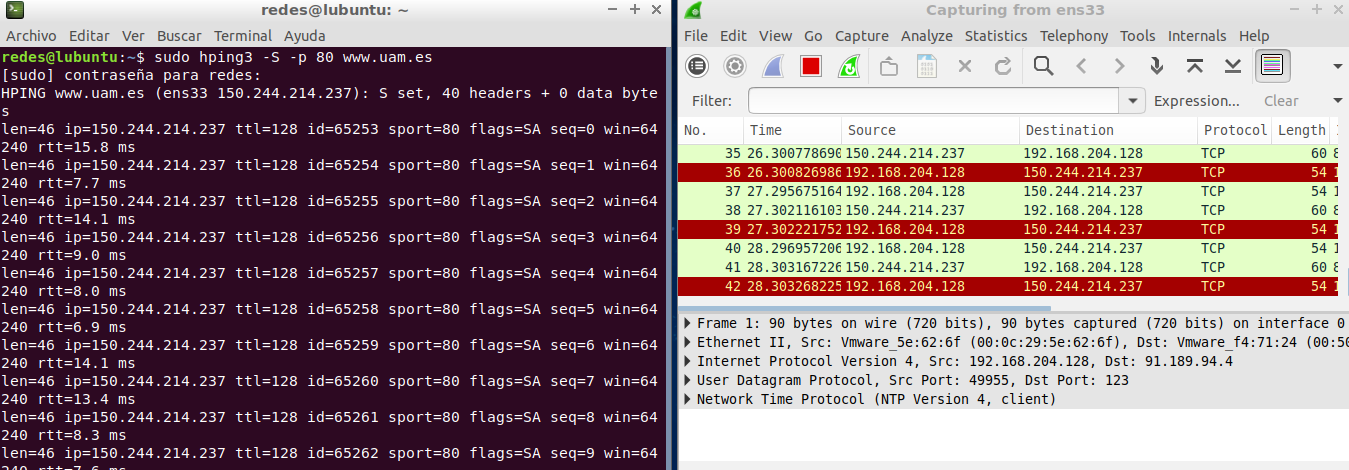
\includegraphics[scale=0.35]{ej1_1.png}
    \caption{Ordenando por la columna PO.}
\end{figure}

Guardamos los paquetes en un fichero y reiniciamos Wireshark.\\ Añadimos las columnas PO (Src port (unresolved)) y PD (Dst port (unresolved)), y ordenamos las entradas por PO. Nótese que compara los datos de PO como si fueran cadenas de texto, y no como si fueran números, así que el resultado 45 iría antes que el 5.

\begin{figure}[h!]
    \centering
    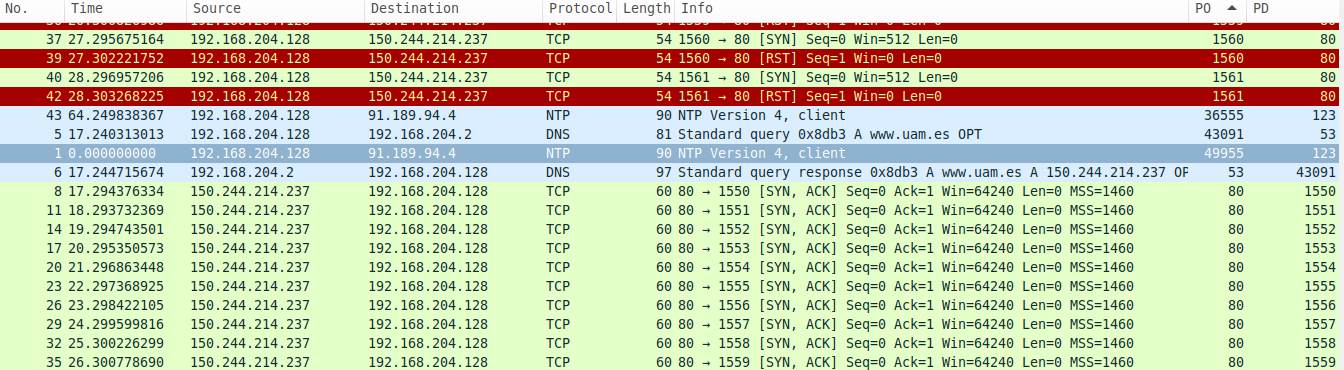
\includegraphics[scale=0.35]{ej1_2.png}
    \caption{Capturando paquetes creados por el comando hping3.}
\end{figure}


\section{Apartado 2}
\subsection{}
El filtro que se ha realizado para que se muestren los paquetes tipo IP con una longitud de paquete mayor que 1000 B es:
$$ip\; and\; ip.len > 1000$$
Guardamos la captura en practica1.pcap.

\subsection{}
Para guardar los paquetes filtrados se exportan en formato pcap.
\begin{figure}[h!]
    \centering
    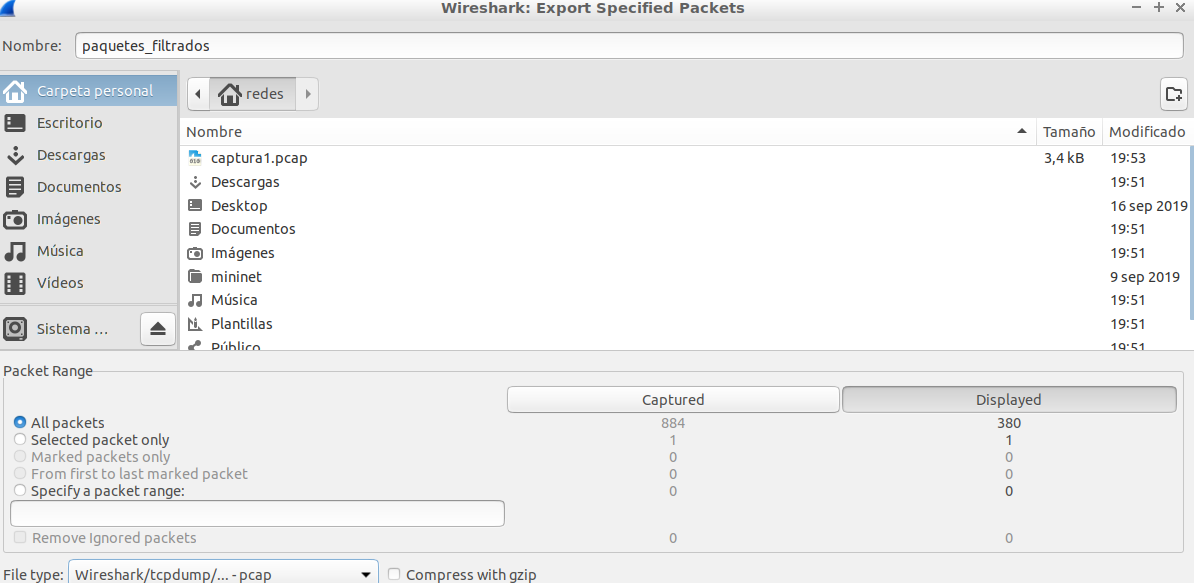
\includegraphics[scale=0.35]{ej2_1.png}
    \caption{Exportar los paquetes mostrados.}
\end{figure}

\subsection{}
La length del paquete IP primero es de 1514, mientras que la length del protocolo IP primero es de 1500, lo que nos dice que hay unos 14 bits de más en el paquete, los que le corresponden a la cabecera del protocolo Ethernet.
\begin{figure}[h!]
    \centering
    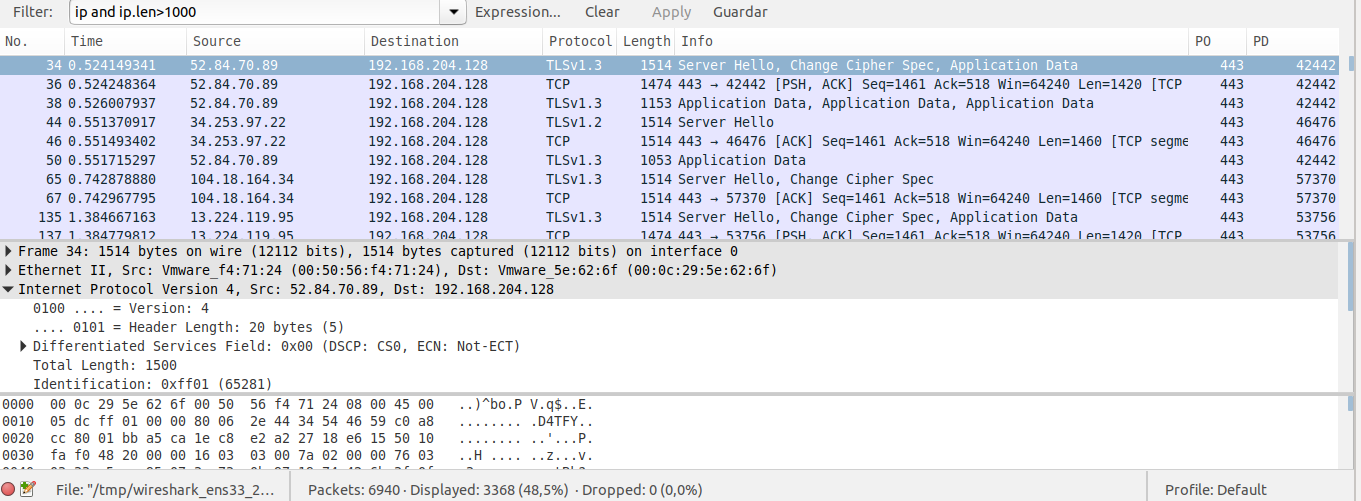
\includegraphics[scale=0.35]{ej2_2.png}
    \caption{Paquetes filtrados.}
\end{figure}
\newpage
\section{Apartado 3}
Para añadir la columna interarrival se han seguido los siguientes pasos: primero vamos al menú \textit{‘Edit$\xrightarrow[]{}$Preferences’}, y en la ventana que aparece se selecciona la opción de \textit{‘User Interface$\xrightarrow[]{}$ Columns’}. En la parte inferior de esta ventana, apretamos al botón de \textit{‘+Añadir’} y en el campo \textit{‘Field Type’} se pone \textbf{‘delta time’}. \\

\begin{figure}[h!]
    \centering
    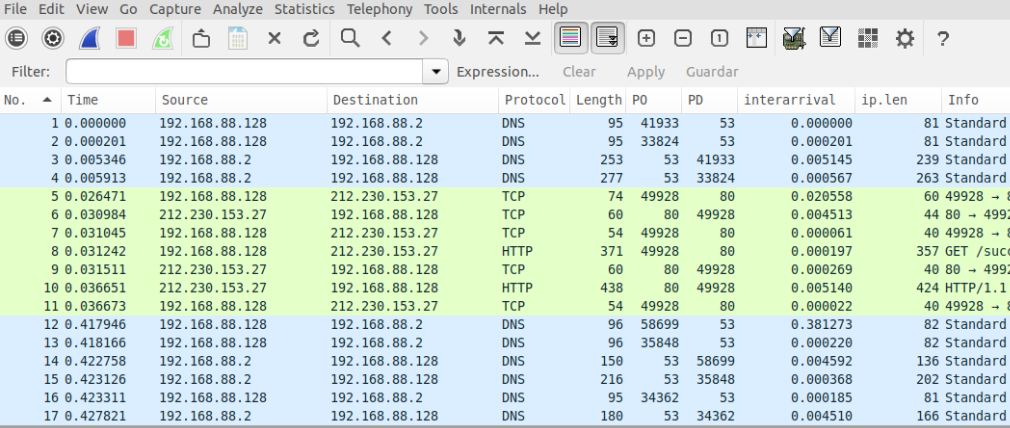
\includegraphics[scale=0.85]{ej3_recorte.PNG}
    \caption{Captura con la columna 'interarrival'.}
\end{figure}

\section{Apartado 4}
Para cambiar el formato de los datos de la columna Time, hay que realizar los pasos del apartado anterior hasta la selección de \textit{‘User Interface$\xrightarrow[]{}$ Columns’}. Una vez en esta ventana, pinchamos sobre la fila de \textit{‘Time’} y cambiamos el \textit{‘Field Type’} de \textbf{‘time’} a \textbf{‘absolute time’}.
\newline
\hspace*{0.5 cm}Este último formato contiene la hora y la resolución en segundos, como se puede ver en la siguiente imagen.
\newline

\begin{figure}[h!]
    \centering
    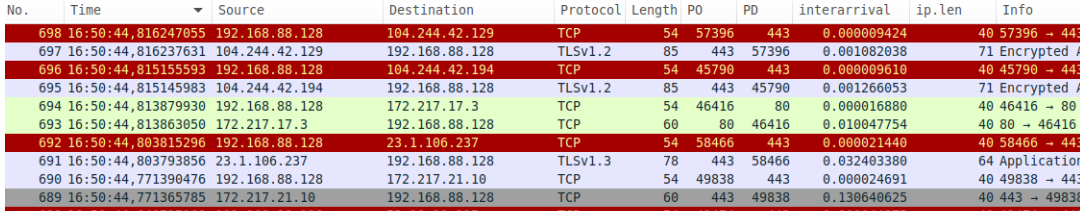
\includegraphics[scale=0.8]{ej4_recorte.PNG}
    \caption{Captura con la fecha y la resolución en segundos.}
\end{figure}

\section{Apartado 5}
Para que le tráfico de solo capture los paquetes de tipo UDP, antes de darle a ‘Start’, en el menú \textit{‘Capture Options’}, en el campo de \textit{‘Capture Filter’} ponemos ‘UDP only’.
\newline
La siguiente captura refleja el resultado de este apartado.

\begin{figure}[h!]
    \centering
    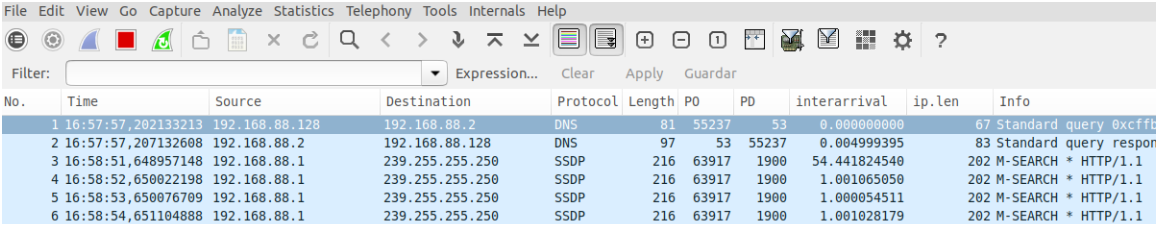
\includegraphics[scale=0.75]{ej5_recorte.PNG}
    \caption{Captura con paquetes de tipo UDP.}
\end{figure}

\end{document}

